\documentclass[convert={density=1200}]{standalone}
\usepackage{tikz}
\usetikzlibrary{shapes.geometric, arrows}

\tikzstyle{server} = [rectangle, rounded corners, text centered, draw=black, fill=green!30, inner sep=5pt]
\tikzstyle{node} = [rectangle, rounded corners, text centered, draw=black, fill=blue!30, inner sep=5pt]
\tikzstyle{action} = [rectangle, text centered, draw=black, inner sep=5pt]
\tikzstyle{trait} = [trapezium, text centered, draw=black, fill=yellow!30, inner sep=5pt, text=red]

\tikzstyle{server_message} = [thick, ->, >=stealth]
\tikzstyle{node_message} = [blue, dashed, ->, >=stealth]
\tikzstyle{action_step} = [green, ->, >=stealth]

\begin{document}

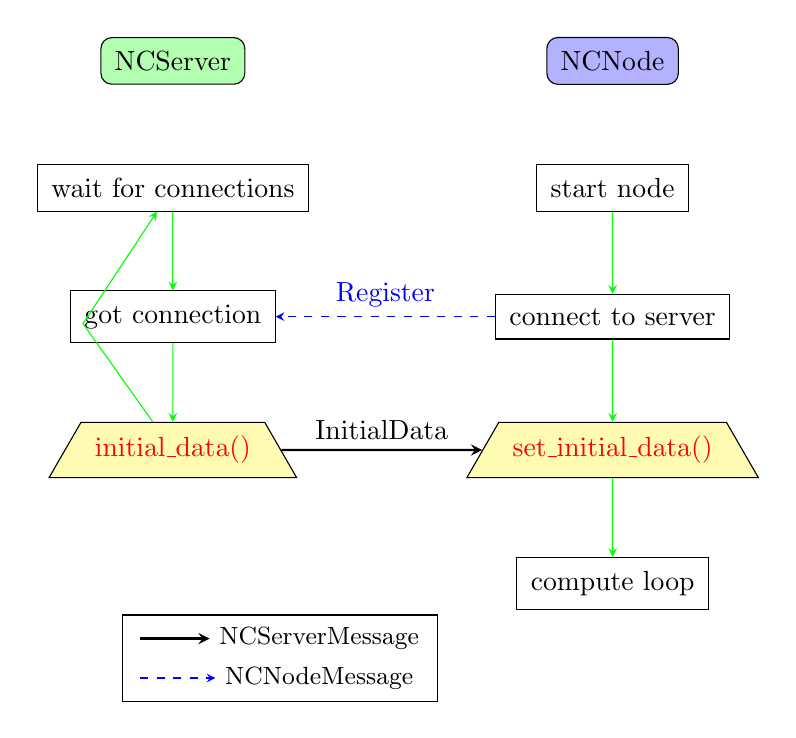
\begin{tikzpicture}

    \matrix [column sep = 20mm, row sep = 10mm] {
        \node (ncserver) [server] {NCServer}; &
        \node (ncnode) [node] {NCNode}; \\

        \node (wait) [action] {wait for connections}; &
        \node (start) [action] {start node}; \\

        \node (connected) [action] {got connection}; &
        \node (connect) [action] {connect to server}; \\

        \node (initial) [trait] {initial\_data()}; &
        \node (set_initial) [trait] {set\_initial\_data()}; \\

        & \node (loop) [action] {compute loop}; \\
    };

    \draw [action_step] (wait) -- (connected);
    \draw [action_step] (connected) -- (initial);

    \draw [action_step] (start) -- (connect);
    \draw [action_step] (connect) -- (set_initial);
    \draw [action_step] (set_initial) -- (loop);

    \draw [node_message] (connect) -- node [above] {Register} (connected);
    \draw [server_message] (initial) -- node [above] {InitialData} (set_initial);

    \draw [action_step] (initial) -- (-4,0) -- (wait);


    \draw [white] (-1, -4.9) rectangle (1, -4.8);

    \draw (-3.5, -4.8) rectangle (0.5, -3.7);

    \node (label1a) at (-3.4, -4) {};
    \node [font=\small] (label1b) at (-1, -4) {NCServerMessage};

    \draw [server_message] (label1a) -- (label1b);

    \node (label2a) at (-3.4, -4.5) {};
    \node [font=\small] (label2b) at (-1, -4.5) {NCNodeMessage};

    \draw [node_message] (label2a) -- (label2b);

\end{tikzpicture}

\end{document}
